\documentclass{article}
\usepackage{times}
\usepackage{graphicx}
\usepackage{subfigure} 
\usepackage{natbib}
\usepackage{algorithm}
\usepackage{algorithmic}
\usepackage{subfigure}
\usepackage{hyperref}
\newcommand{\theHalgorithm}{\arabic{algorithm}} % Fixes misbehavior of conflicting packages.
\usepackage{icml2016/icml2016} 

\icmltitlerunning{Approximate State Abstraction}

% --- Note Commands ---
\usepackage{color}
\newcommand\dnote[1]{\textcolor{blue}{Dave: #1}}
\newcommand\enote[1]{\textcolor{green}{Ellis: #1}}

% --- DOCUMENT ---
\begin{document}

\twocolumn[
\icmltitle{Approximate State Abstraction}

% Paper Meta Info
\icmlauthor{David Abel}{david_abel@brown.edu}
\icmladdress{Brown University,
            115 Waterman Street, Providence, RI 02906}
\icmlauthor{D. Ellis Hershkowitz}{david_hershkowitz@brown.edu}
\icmladdress{Brown University,
            115 Waterman Street, Providence, RI 02906}
\icmlauthor{Michael L.\ Littman}{michael_littman@brown.edu}
\icmladdress{Brown University,
            115 Waterman Street, Providence, RI 02906}
    
\icmlkeywords{Reinforcement Learning, State Aggregation, State Abstraction, Planning, MDP}
            
\vskip 0.3in
]


% --- ABSTRACT ---
\begin{abstract}
The combinatorial explosion that plagues planning and reinforcement-learning algorithms can be reversed using abstraction. For instance, prohibitively difficult task representations can be condensed so that solutions are tractably computable. In this work, we investigate a theoretical framework for approximate state abstraction that preserves near optimal behavior. Reinforcement learning agents using these abstractions may treat experiences that resemble each other as equivalent, and generalize knowledge to novel scenarios based on prior experiences. We present theoretical guarantees of the quality of value functions derived from four classes of approximate state abstraction. Additionally, we empirically evaluate the relationship between the degree of approximation and the degree of abstraction achieved, as well as the tradeoff between approximation magnitude and optimality of behavior.
\end{abstract}

% Set of actions within epsilon (Q*) is the same for two states? Better than boltzmann.


% --- SECTION: Introduction ---
\section{Introduction}

\begin{itemize}
\item Solving MDPs is P-Complete, where the dominant factor is $|\mathcal{S}|$.
\item Sample complexity is {\it also} dominated by $|\mathcal{S}|$.
\item To make MDPs with large $|\mathcal{S}|$ tractable, we can reduce the MDPs to a simpler form.
\item In this work, we show that compressing MDPs in a particular way allows for the transfer of bounded-error solutions between the compressed MDP and ground MDP.
\item Q: Why approximate?
\item A: Approximate can compress strictly more than compression based on equality
\item A: Approximate compression requires the type of knowledge that we could imagine learning (i.e.. approximate knowledge)
\end{itemize}

% --- SECTION: Background ---
\section{Background}

\subsection{MDP/RL}

\subsection{Lihong Li}

% Quick MDP blurb?

% Phi notation

% Evluation of Abstract MDP

% Abstract MDP, Ground MDP, Homogenizing Gun

% Previous state aggregation stuff? Or should be in related work?


% --- SECTION: Related Work ---
\section{Related Work}

% Approximate abstraction work.
%Dean: 
%\begin{itemize}
%\item \citep{dean1997model} Does abstraction with model equality.
%\item \citep{dean1997modelmin} Does approximate abstraction with model similarity.
%\end{itemize}
%
%Boutilier:
%\begin{itemize}
%\item ~\citep{dearden1997abstraction} Abstraction: a similar ish bound with a similar is agenda.
%\item ~\citep{Boutilier2000} Stochastic DP: tree based policies, sort of bound thingies.
%\end{itemize}
%
%Even~\cite{even2003approximate}: COLT paper on different metrics
%
%Ortner:
%\begin{itemize}
%\item ~\cite{ortner2013adaptive}: Uses Dean results to do UCRL online learning of abstraction. 
%\item ~\cite{odalric2013optimal}: Learn which abstraction to use online (similar to the Nan paper)
%\end{itemize}


\subsection{Approximate State Abstraction}
\citep{dean1997modelmin} investigates partitioning an MDP's state space into $\epsilon$-homogenous blocks, which are defined as clusters of states whose transition model and reward function are within $\epsilon$ of each other. They provide bounds on the error incurred as a result of using the optimal policy defined over these blocks in the original MDP. This method of abstraction is effectively characterized as a function belonging to the approximate class $\phi_{model}$.
Several approaches build on the notion of $\epsilon$-homogeneity. ~\citep{even2003approximate} analyze different distant metrics used in the process of identifying $\epsilon$-homogenous partitions. ~\cite{ortner2013adaptive} develops an algorithm for learning partitions in an on line setting by taking advantage of the confidence bounds for $T$ and $R$ provided by UCRL~\cite{auer2009near}.

%Prior work considers abstractions related to transition model similarity, or both transition model and reward function similarity with the aim of reducing the state space size required for planning and learning while still achieving a bounded error solution~\cite{even2003approximate,ortner2013adaptive,Boutilier2000}. All of this work is closely in line with our own agenda; they investigate rules for abstractions that may inform a reduced, abstract MDP, the solution to which has bounded error in the original MDP. However, all prior results explore model similarity abstraction rules, whereas we consider several broader classes of approximate abstraction. Furthermore, our results depend on no assumptions regarding the structure of the MDPs in which we apply our abstraction, and generalize to both the reinforcement learning or the planning setting, while many previous approaches require simplifying assumptions about the space of MDPs\dnote{a comment about what assumptions are made would be nice}, or only work target planning.

\subsection{Specific Abstraction Algorithms}
Many previous works have targeted the creation of algorithms that enable state abstraction for MDPs. \citep{andre2002state} investigates a method for state abstraction in hierarchical reinforcement learning leveraging a programming language called ALISP that promotes the notion of {\it safe} state abstraction. Agents programmed using ALISP can ignore irrelevant parts of the state, achieving abstraction that maintains optimality. ~\cite{dietterich2000hierarchical} develops the MAXQ algorithm, a framework for composing tasks into an abstracted hierarchy. \citep{jong2005state} introduce a method called {\it policy-irrelevance}, in which agents identify (online) which state variables may be safely ignored in a factored MDP, and consequently achieve state abstraction. The agent will learn to ignore state variables that don't impact optimal behavior, and is consequently contained within the approximate $\phi_{a^*}$ work. For a full survey of algorithms that leverage state abstraction in recent reinforcement learning literature, see~\cite{li2006towards}.


% Other? Selecting abstractions
%\subsection{Selecting Abstractions}
%\citep{jiang2015abstraction} investigate the question of choosing between two abstractions during learning. They provide analysis for an online approach to identifying the better abstraction. 

% Defining 

% Critically, our work differs from these in that our primary aim is to achieve understanding of what methods of abstraction in reinforcement learning can maintain bounded error solutions, while these focus on particular strategies that fit within our framework.

% Lihong/Walsh/Littman: Towards a unified theory...

%\begin{itemize}
%\item {\bf Approximate equivalence of MDP}~\cite{even2003approximate}
%\item ALisp~\cite{andre2002state}
%\item Aggregation in DP~\cite{Bean2011}
%\item {\bf Does approximate aggregation and then UCRL}~\cite{ortner2013adaptive}
%Very similar to our overall goal: learn an abstraction function online using confidence bounds as the epsilon. Wowza. Only uses the whole model similarity business though. Seems to be the case for all of the approximate aggregation work (just does the bisimulation or $\epsilon-homogeneity$)
%
%\item Selecting the state rep in RL~\cite{maillard2011selecting}
%\item Near optimal state reps~\cite{ortner2014selecting}
%\item SMDP homomorphisms~\cite{ravindran2003smdp}
%\end{itemize}


% --- SECTION: State Abstraction ---
\section{Approximate State Abstraction}

% Explain each of the Phis

% One theorem, each separate phi is its own lemma.

% Proof of Q^*

% Possibly a lemma for NP-Completeness of the minimal such phi for all abstractions (was a result for model in previous cases).

% Subsections for proofs for each phi
\dnote{Insert lemma for each phi as their subsection, maybe with proof sketch but likely just dump in appendix.}

% Subsection: 

% Subsection: Phi_Q
\subsection{$\phi_{Q^*}$}

% Subsection: Phi_M
\subsection{$\phi_{model}$}

% Subsection: Phi_{Mult}
\subsection{$\phi_{mult}$}

% Subsection: Phi_B
\subsection{$\phi_{bolt}$}

% Subsection: Other Abstractions
\subsection{Other Abstractions}

We note that one natural way of approximating $\phi_{a^*}$ from ~\cite{li2006towards}, in which states that are compressed together share optimal actions and the Q values of these actions are within $\varepsilon$ is ultimately equivalent to the crisp abstraction $\phi_{\pi^*}$, in states that are compressed share an optimal action. A true approximation of $\phi_{a^*}$ ought to also approximate the optimality of each action. Given the degree of compression achievable under $\phi_{a^*}$, especially with temporally extended actions, we foresee this approximate form of abstraction as being of great interest, and plan to investigate it in future work.

We are {\it not} going to provide results for $\phi_{\pi^*}$, since relaxing equality of optimal actions doesn't mean anything.

Additionally, we are {\it not} going to provide results for $\phi_{Q^\pi}$, since as Lihong's paper notes, ``It is an open question how to find $Q^\pi$ irrelevance abstractions without enumerating all possible policies, they do not give results. Furthermore, an MDP for which this is true is an awfully weird MDP...

Lastly, we are interested in a generalization of $\phi_{mult}$  and $\phi_{bolt}$ that handles a broader space of distributions over Q values.


% Some abstractions DON'T preserve a meaningful notion of optimality.



% --- SECTION: Example Domains ---
\section{Example Domains}

\dnote{For each section, we'll include a plot comparing $\epsilon$ to \# states, and $\epsilon$ to performance. For UpWorld and NChain, we can include visuals of uncompressed and compressed (not useful for trench).}

% Subsection: UpWorld
\subsection{UpWorld}

\dnote{As part of UpWorld we can include the result about the unbounded improvement in sample complexity (small lemma or something?)}

% Insert visual and/or stats on number of states and performance of VI solving the abstract MDP and evaluating the resulting policy on the original MDP


% Subsection: NChain
\subsection{NChain}

% Insert visual and/or stats on number of states and performance of VI solving the abstract MDP and evaluating the resulting policy on the original MDP


% Subsection: Trench
\subsection{Trench}

% Insert visual and/or stats on number of states and performance of VI solving the abstract MDP and evaluating the resulting policy on the original MDP


% Figure: The Trench Problem
\begin{figure}[h]
\centering
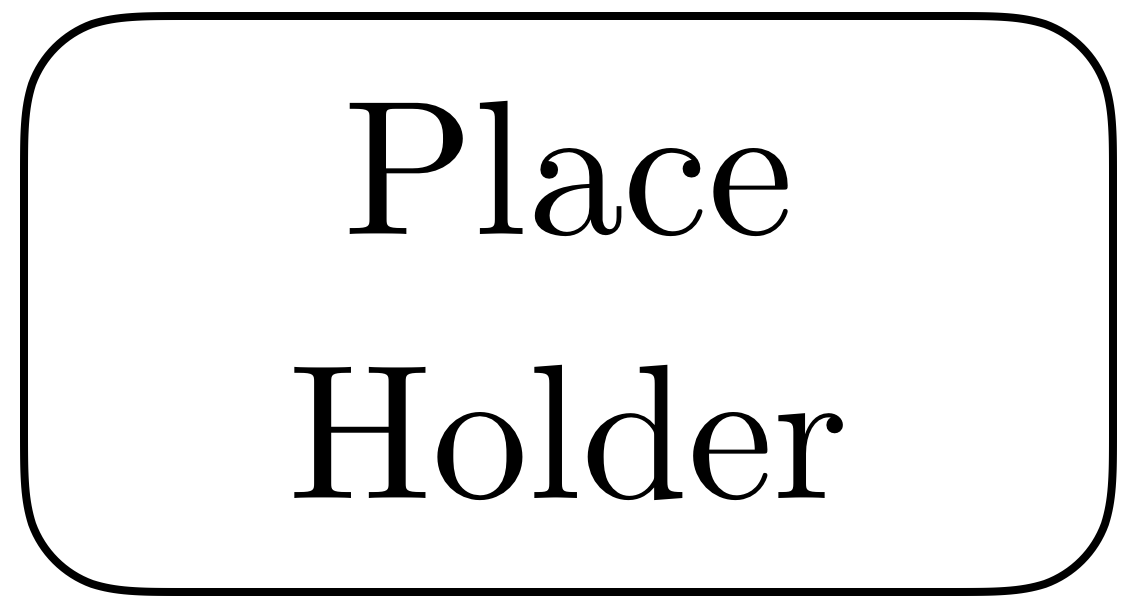
\includegraphics[width=0.42\columnwidth]{figures/placeholder.png}
\caption{The Trench Problem}
\label{fig:trench}
\end{figure}


% --- SECTION: Approximate Abstraction on Example Domains ---
\section{Approximate Abstraction on Example Domains}

% Figure: Epsilon vs. #States for all three sample domains.
\begin{figure}
\subfigure[UpWorld]{
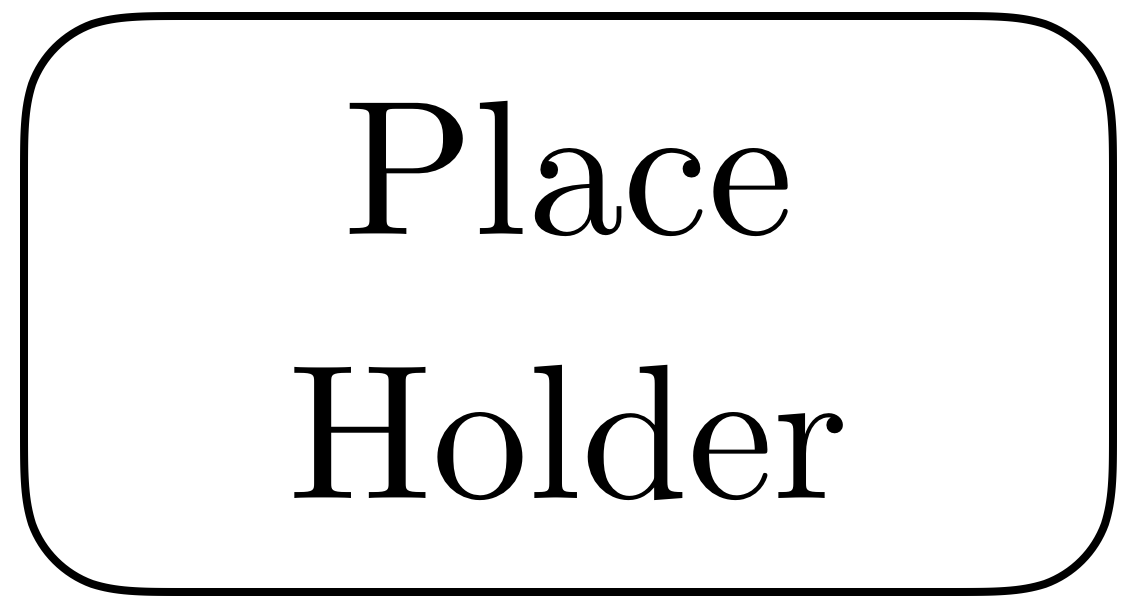
\includegraphics[width=0.28\columnwidth]{figures/placeholder.png}}
\subfigure[NChain]{
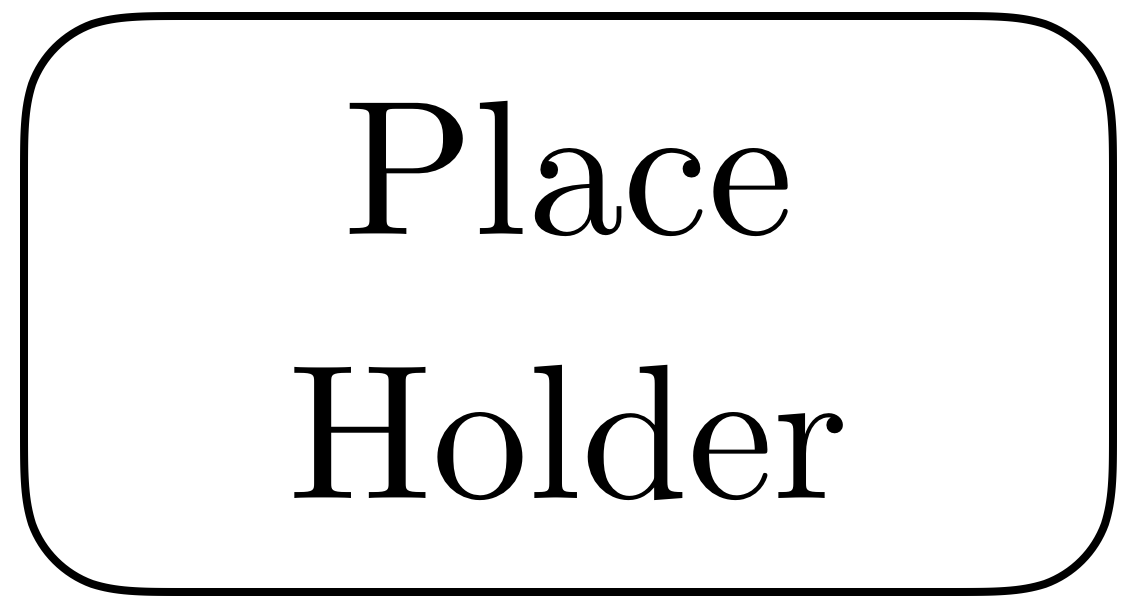
\includegraphics[width=0.28\columnwidth]{figures/placeholder.png}}
\subfigure[Trench]{
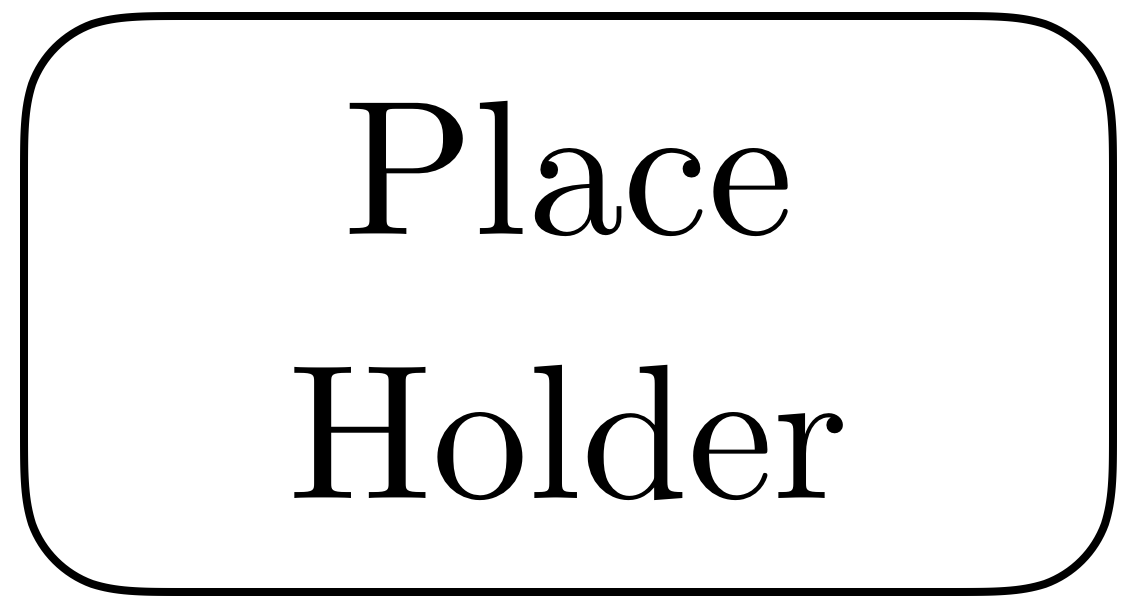
\includegraphics[width=0.28\columnwidth]{figures/placeholder.png}}
\label{fig:eps-states}
\caption{$\epsilon$ vs. Num States}
\end{figure} 

% Figure: Epsilon vs. Error in Abstract Value Function
\begin{figure}
\subfigure[UpWorld]{
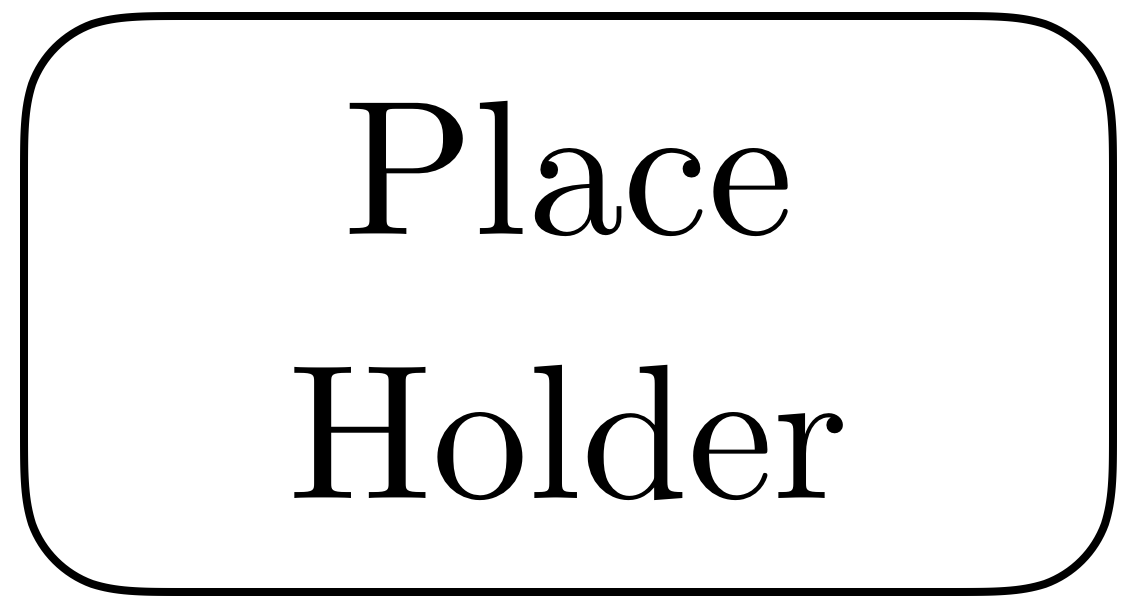
\includegraphics[width=0.28\columnwidth]{figures/placeholder.png}}
\subfigure[NChain]{
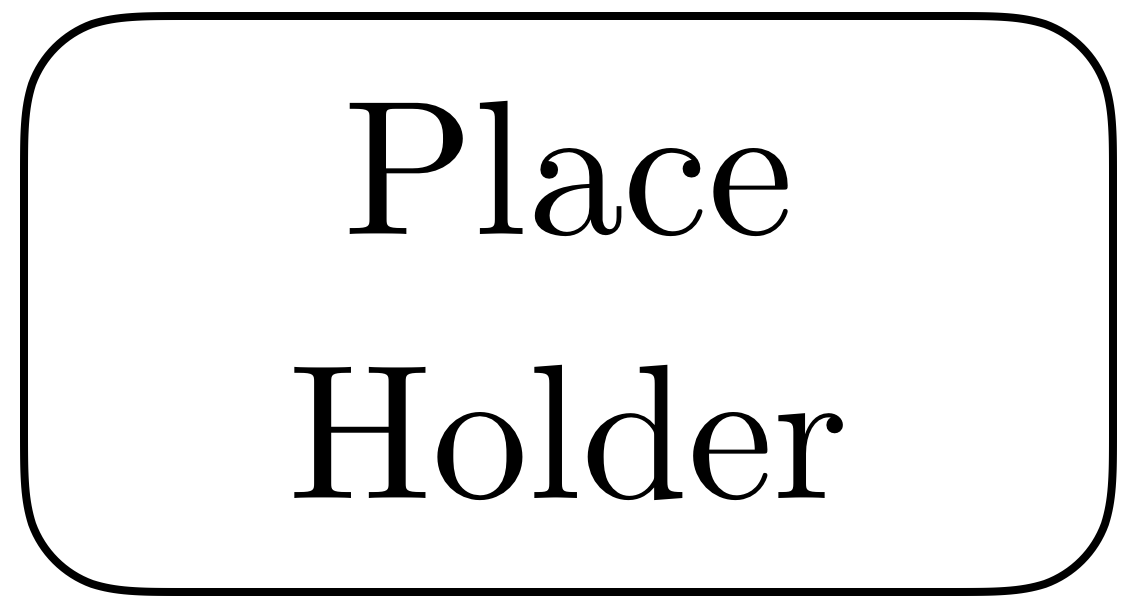
\includegraphics[width=0.28\columnwidth]{figures/placeholder.png}}
\subfigure[Trench]{
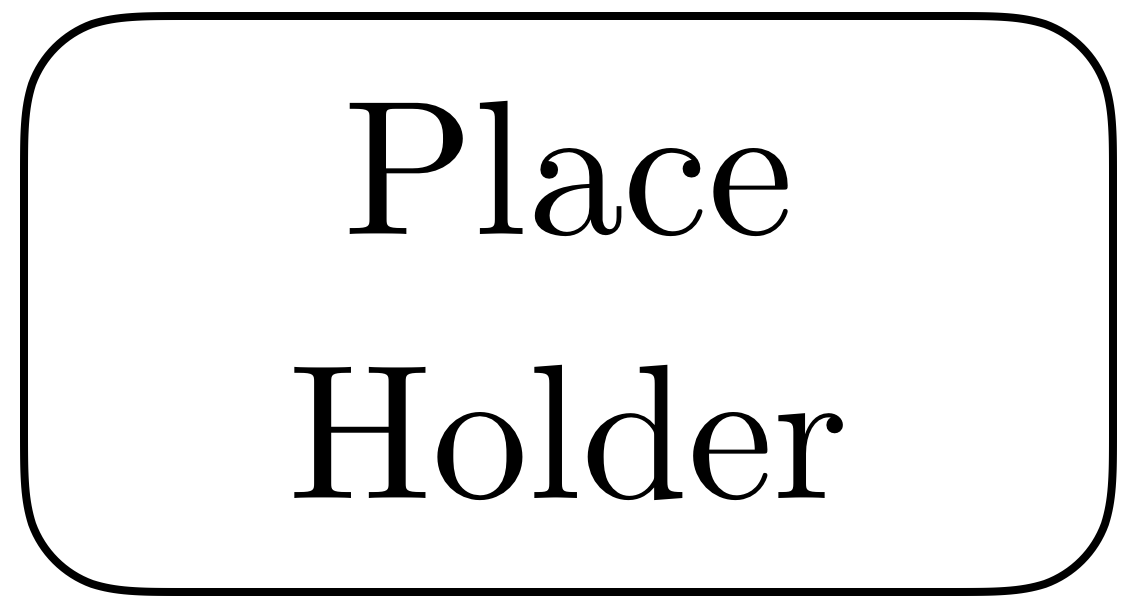
\includegraphics[width=0.28\columnwidth]{figures/placeholder.png}}
\label{fig:eps-states}
\caption{$\epsilon$ vs. Error in Abstract Value Function}
\end{figure} 



% Subsection: Abstract Domain Visualizations
\subsection{Abstract Domain Visualizations}

% Figure: UpWorld MDP visuals
\begin{figure}[h]
\centering
\subfigure[UpWorld]{
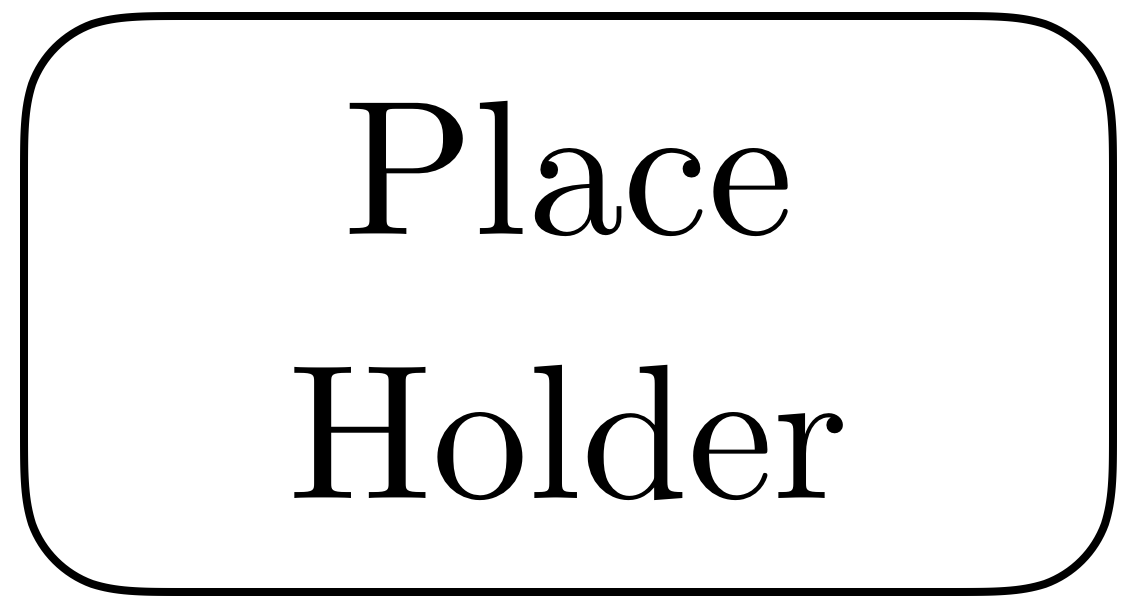
\includegraphics[width=0.46\columnwidth]{figures/placeholder.png}}
\hspace{3mm}
\subfigure[Abstracted UpWorld]{
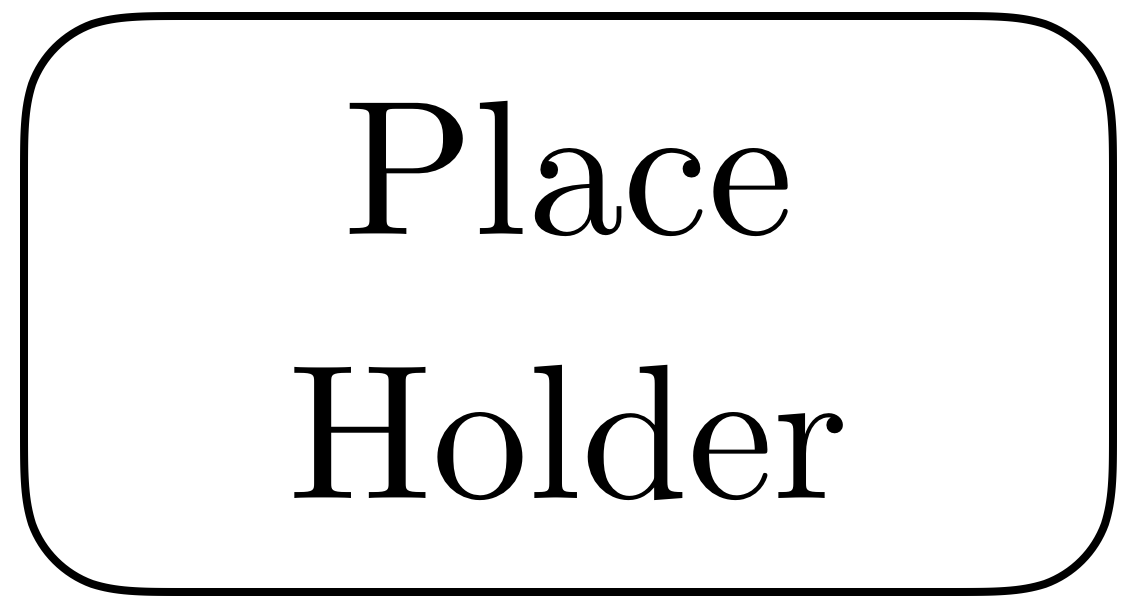
\includegraphics[width=0.46\columnwidth]{figures/placeholder.png}}
\caption{Visualization of Original UpWorld vs. Abstracted UpWorld}
\end{figure}

% Figure: NChain MDP visuals
\begin{figure}[h]
\centering
\subfigure[NChain]{
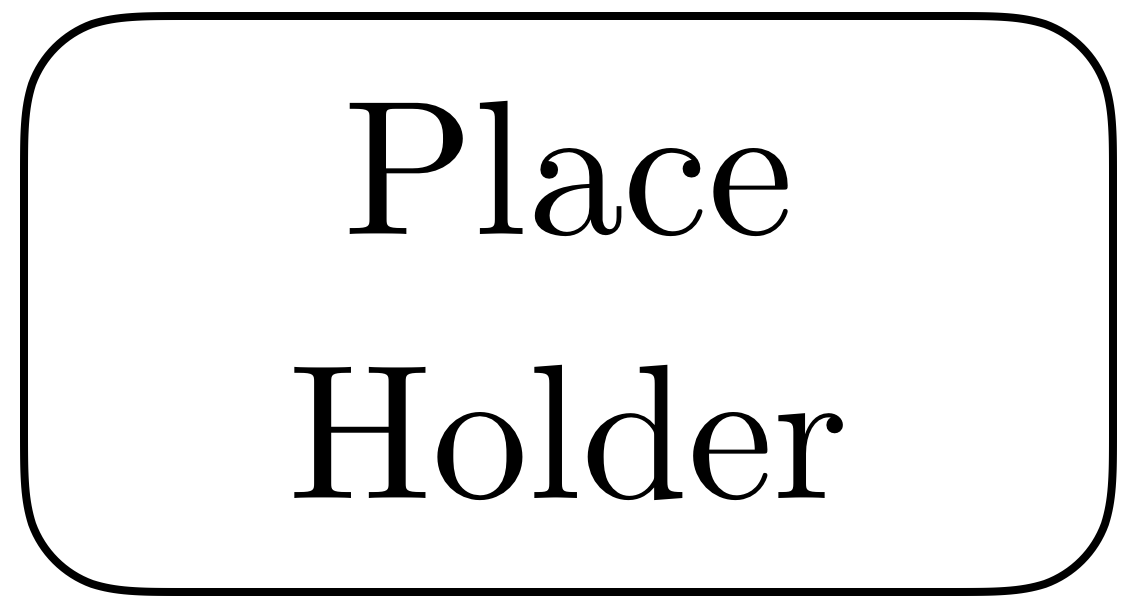
\includegraphics[width=0.46\columnwidth]{figures/placeholder.png}}
\hspace{3mm}
\subfigure[Abstracted NChain ]{
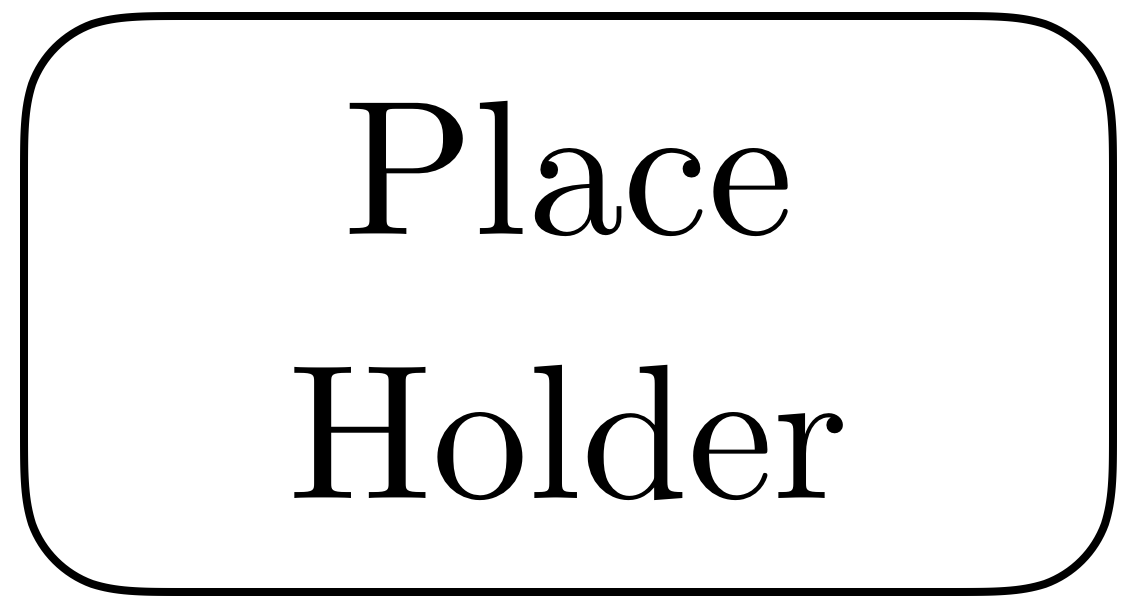
\includegraphics[width=0.46\columnwidth]{figures/placeholder.png}}
\caption{Visualization of Original NChain vs. Abstracted NChain}
\end{figure}






% --- SECTION: Conclusion ---
\section{Conclusion}

% Summary

% Future Work
\begin{enumerate}
\item Learning Phi
\begin{itemize}
\item Exploration vs. Exploitation problem is different while trying to learn Phi
\end{itemize}
\item Compressibility
\begin{itemize}
\item Relationship between approximate abstract and compressibility
\end{itemize}
\item POMDP and abstraction
\end{enumerate}





% --- BIBLIOGRAPHY ---
\bibliographystyle{icml2016/icml2016}
\bibliography{state_abs}

\end{document}
